\documentclass[../main.tex]{subfiles}

\begin{document}


\practica{Periféricos mapeados en memoria (MMIO): Entrada/Salida de propósito general (GPIO)}

    \subsection{Objetivos}
        \begin{itemize}
            \item Comprender el concepto de \textbf{Memory-Mapped I/O (MMIO)}.
            \item Analizar la organización del mapa de memoria del microcontrolador \MCU.
            \item Aprender a manipular directamente los registros de entrada/salida mediante máscaras de bits en C.
        \end{itemize}

    \subsection{Fundamentos teóricos}
        En un procesador de propósito general, numerosas funciones se realizan a través de \textit{periféricos}, componentes anexos al procesador con funciones específicas. 

        En la arquitectura ARM, los periféricos no se controlan con instrucciones dedicadas, sino que se comunican con la CPU a través del bus del sistema (\textit{AXI-AHB Bus Matrix}) asignándoles direcciones físicas dentro del mapa de memoria de 32 bits (4GB).
    
        Cada periférico posee un conjunto de \textbf{registros de control, estado y datos} ubicados en direcciones consecutivas a partir de una dirección base (\textit{Base Address}). Escribiendo y leyendo en esas direcciones, conseguimos comunicarnos con los periféricos, que a su vez se conectarán con los diferentes pines del procesador. Los pines servirán para su conexión con el exterior con otros elementos, como LEDs, botones, pantallas, puertos, etc.

        \begin{figure}[htbp]
        \centering
        \begin{tikzpicture}[
            node distance = 1.2cm and 0.8cm,
            box/.style = {
            draw=gray!80, 
            thick, 
            rounded corners=6pt, 
            fill=white, 
            align=center, 
            inner sep=8pt,
            font=\small,
            minimum height=1.2cm
            },
            arrow/.style = {
            -{Stealth[scale=1.2]}, 
            thick, 
            draw=gray!80
            },
            labelstyle/.style = {
            font=\tiny\sffamily, 
            color=gray!90, 
            above
            }
        ]

            % Nodos
            \node [box, fill=blue!5] (cpu) {
            \textbf{CPU ARM}\\[-2pt]
            \tiny(Ejecuta código C)
            };

            \node [box, fill=blue!10, right=of cpu] (periph) {
            \textbf{Periférico}\\[-2pt]
            \tiny(GPIO / Registros MMIO)
            };

            \node [box, fill=yellow!10, right=of periph] (pin) {
            \textbf{Pin Físico}\\[-2pt]
            \tiny(e.g. PA7)
            };

            \node [box, fill=green!10, right=of pin] (ext) {
            \textbf{Comp. Externo}\\[-2pt]
            \tiny(e.g. LED5 / Botón)
            };

            % Conexiones con etiquetas descriptivas
            \draw [arrow] (cpu) -- node[labelstyle] {Bus de Sistema} (periph);
            \draw [arrow] (periph) -- node[labelstyle] {Señal Interna} (pin);
            \draw [arrow] (pin) -- node[labelstyle] {Conexión Placa} (ext);

        \end{tikzpicture}
        \caption{Flujo de control desde el código en CPU hasta el componente exterior a través de MMIO.}
        \label{fig:diagrama_mmio}
        \end{figure}

        En nuestro caso, disponemos de un procesador \MCU. Podemos consultar el manual de referencia \REFMAN para ver una lista completa de sus periféricos y las direcciones de memoria donde se ubican sus registros. La sección \REFMAN[1.6] detalla todo este mapa de memoria, que se muestra en las \Cref{fig:stm32f723mm,fig:stm32f723mm_detail}

        \begin{figure}
            \centering
            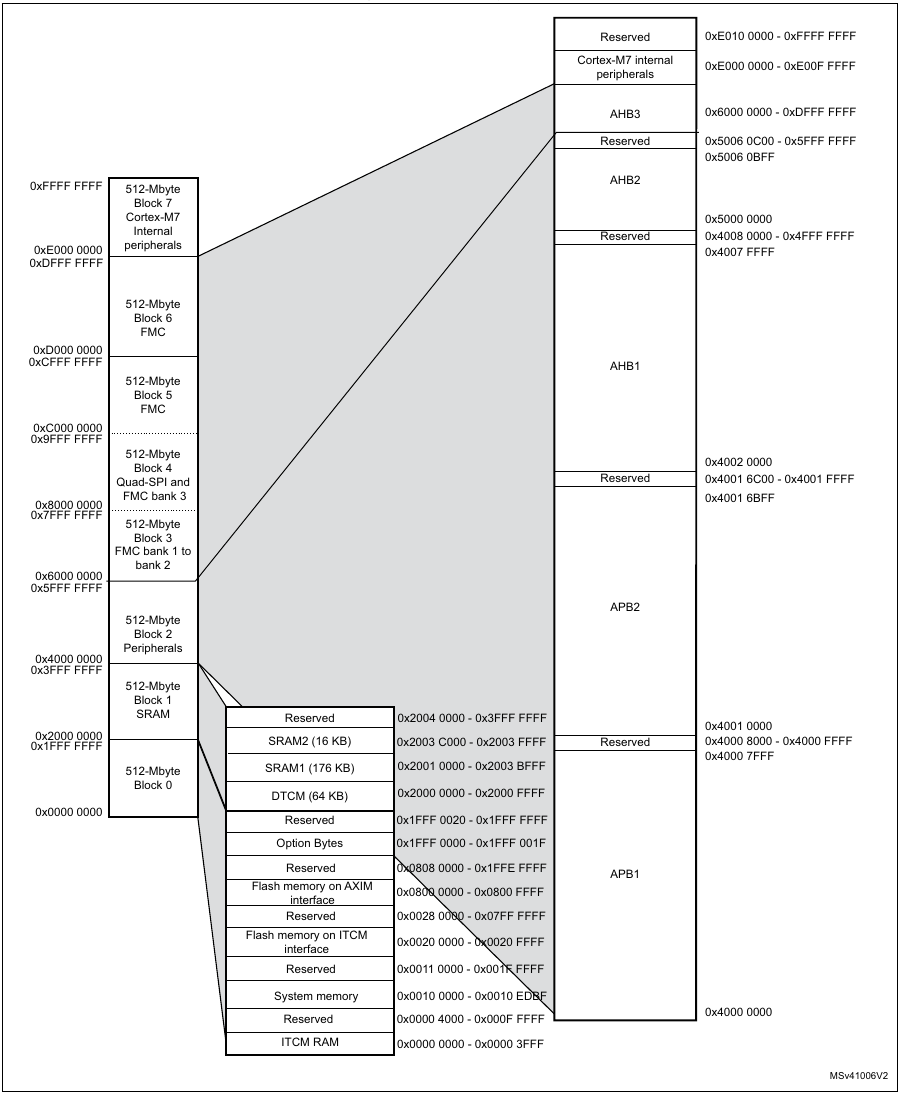
\includegraphics[width=\textwidth]{res/stm32f723mm.png}
            \caption{Mapa de memoria del \MCU}
            \label{fig:stm32f723mm}
        \end{figure}

        \begin{figure}
            \centering
            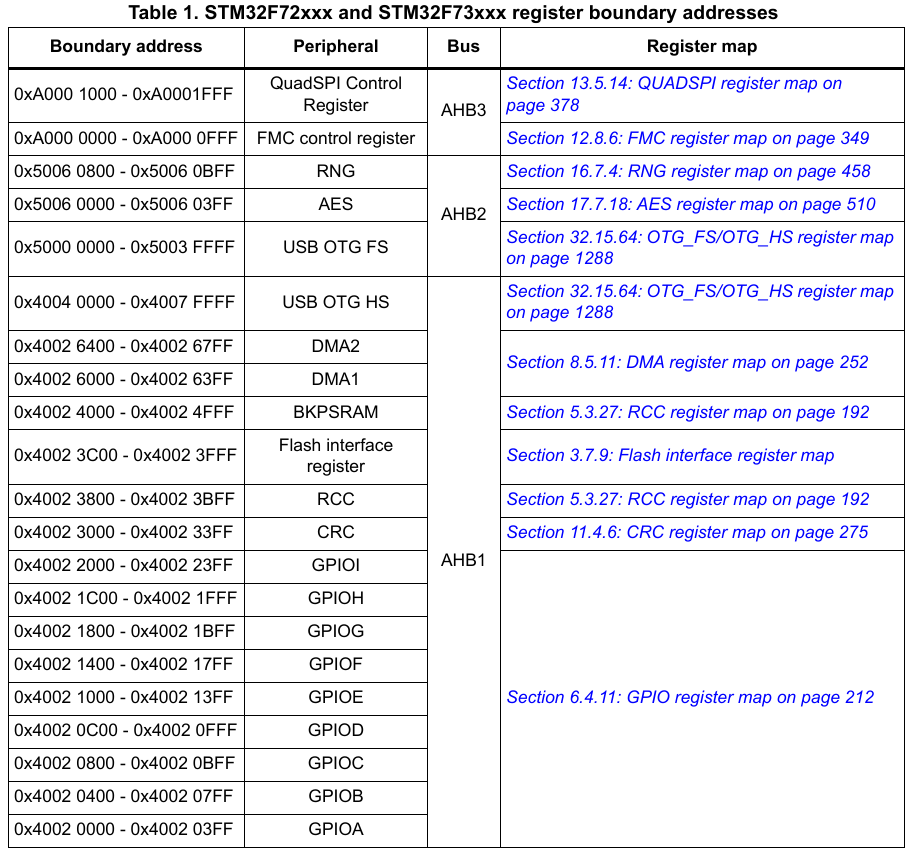
\includegraphics[width=\textwidth]{res/stm32f723mm_detail.png}
            \caption{Detalle del mapa de memoria del \MCU}
            \label{fig:stm32f723mm_detail}
        \end{figure}

        De aquí ya podemos deducir las direcciones de los diferentes controladores de GPIO. Vemos que están nombrados con letras (desde GPIOA hasta GPIOI). Por ejemplo, el controlador de GPIOA está en la dirección \MEMORY{0x40020000}. ¿Pero claro, cómo lo manejamos? Para ello debemos conocer todos los registros que se encuentran en esa zona de memoria. Esa información la tenemos en \REFMAN[6.4]. 

        A modo de ejemplo, se muestra en la \Cref{fig:stm32f723mm_moder} la información referente al registro \REG{MODER} del controlador de GPIO. Observamos que, en una palabra de 32 bits, contiene la configuración de modo de pin (Input/Output/Función alternativa/Analógico) para hasta 16 pines diferentes. Es decir, utiliza 2 bits para la configuración de cada pin. Los dos bits menos significativos corresponden al pin 0, y los 2 más significativos al pin 15, con el resto entre medias. Escribiendo en este registro configuraremos el modo de cada uno de estos pines.

        \begin{figure}
            \centering
            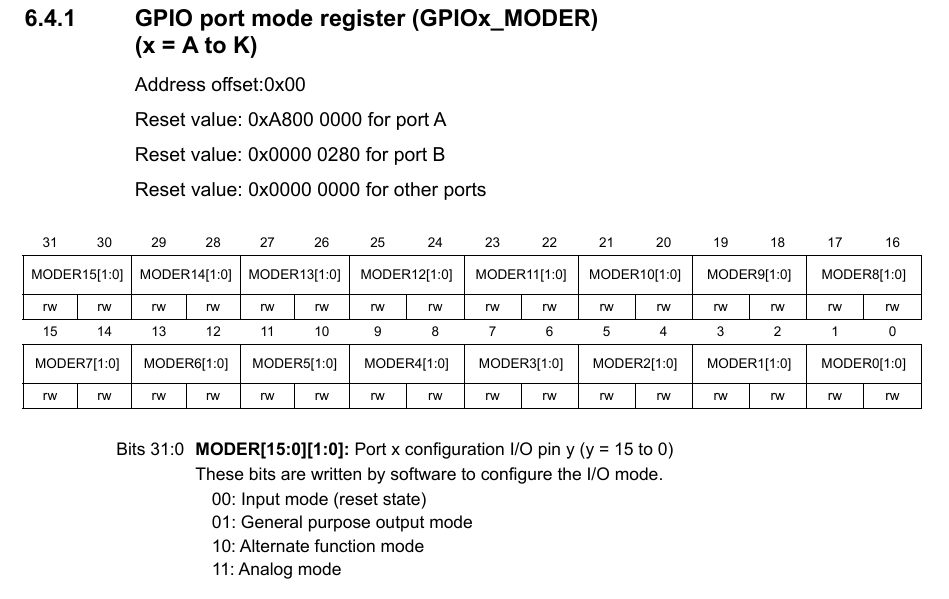
\includegraphics[width=\textwidth]{res/stm32f723_gpio_moder_reg.png}
            \caption{Detalle del registro MODER}
            \label{fig:stm32f723mm_moder}
        \end{figure}

        Hemos visto pues que podemos configurar ciertos puertos de entrada/salida, que a su vez cuentan con numerosos pines. Pero, ¿en qué puerto/pin se sitúa, por ejemplo, un LED?. Para ello, debemos acudir a la documentación de la placa, donde se han diseñado físicamente las conexiones desde el procesador, hasta los diferentes elementos de soporte. En concreto, en la sección \BRDMAN[5.16] tenemos la lista de todas las conexiones de botones y LEDs. Lo vemos en la \Cref{fig:stm32f723disco_pins}

        \begin{figure}
            \centering
            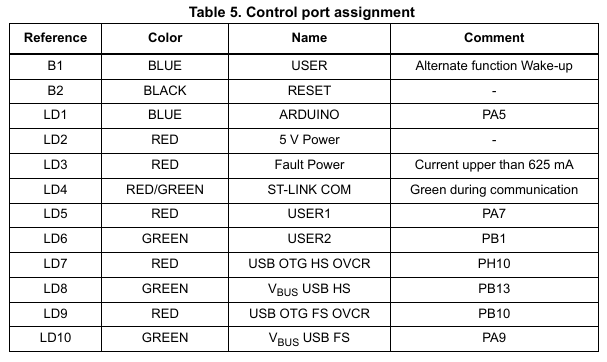
\includegraphics[width=\textwidth]{res/stm32f723_discovery_pins.png}
            \caption{Pines para LEDS y botones de la placa \BOARD}
            \label{fig:stm32f723disco_pins}
        \end{figure}

        Finalmente, sabemos que, por ejemplo, el LED5 se controla desde el puerto GPIOA, en el PIN 7. El puerto A está en la dirección \MEMORY{0x40020000}, y dispone de varios registros que deberemos configurar adecuadamente para controlar, finalmente, el LED.


    \subsection{Desarrollo de la práctica}

        \subsubsection{Creación del proyecto}

            Vamos a controlar, directamente y escribiendo en registros del procesador, un LED (en concreto, el LED5 que acabamos de ver). Pero antes, debemos crear un proyecto en STMCubeIDE, la herramienta de desarrollo de ST. Para ello:
            \begin{enumerate}
                \item Abrimos STM32CubeIDE, buscándolo en el menú del sistema. Elegimos un workspace (o carpeta de trabajo) donde trabajar. Tras abrirlo, veremos el programa de la \Cref{fig:scrn_01_startup}

                    \begin{figure}
                        \centering
                        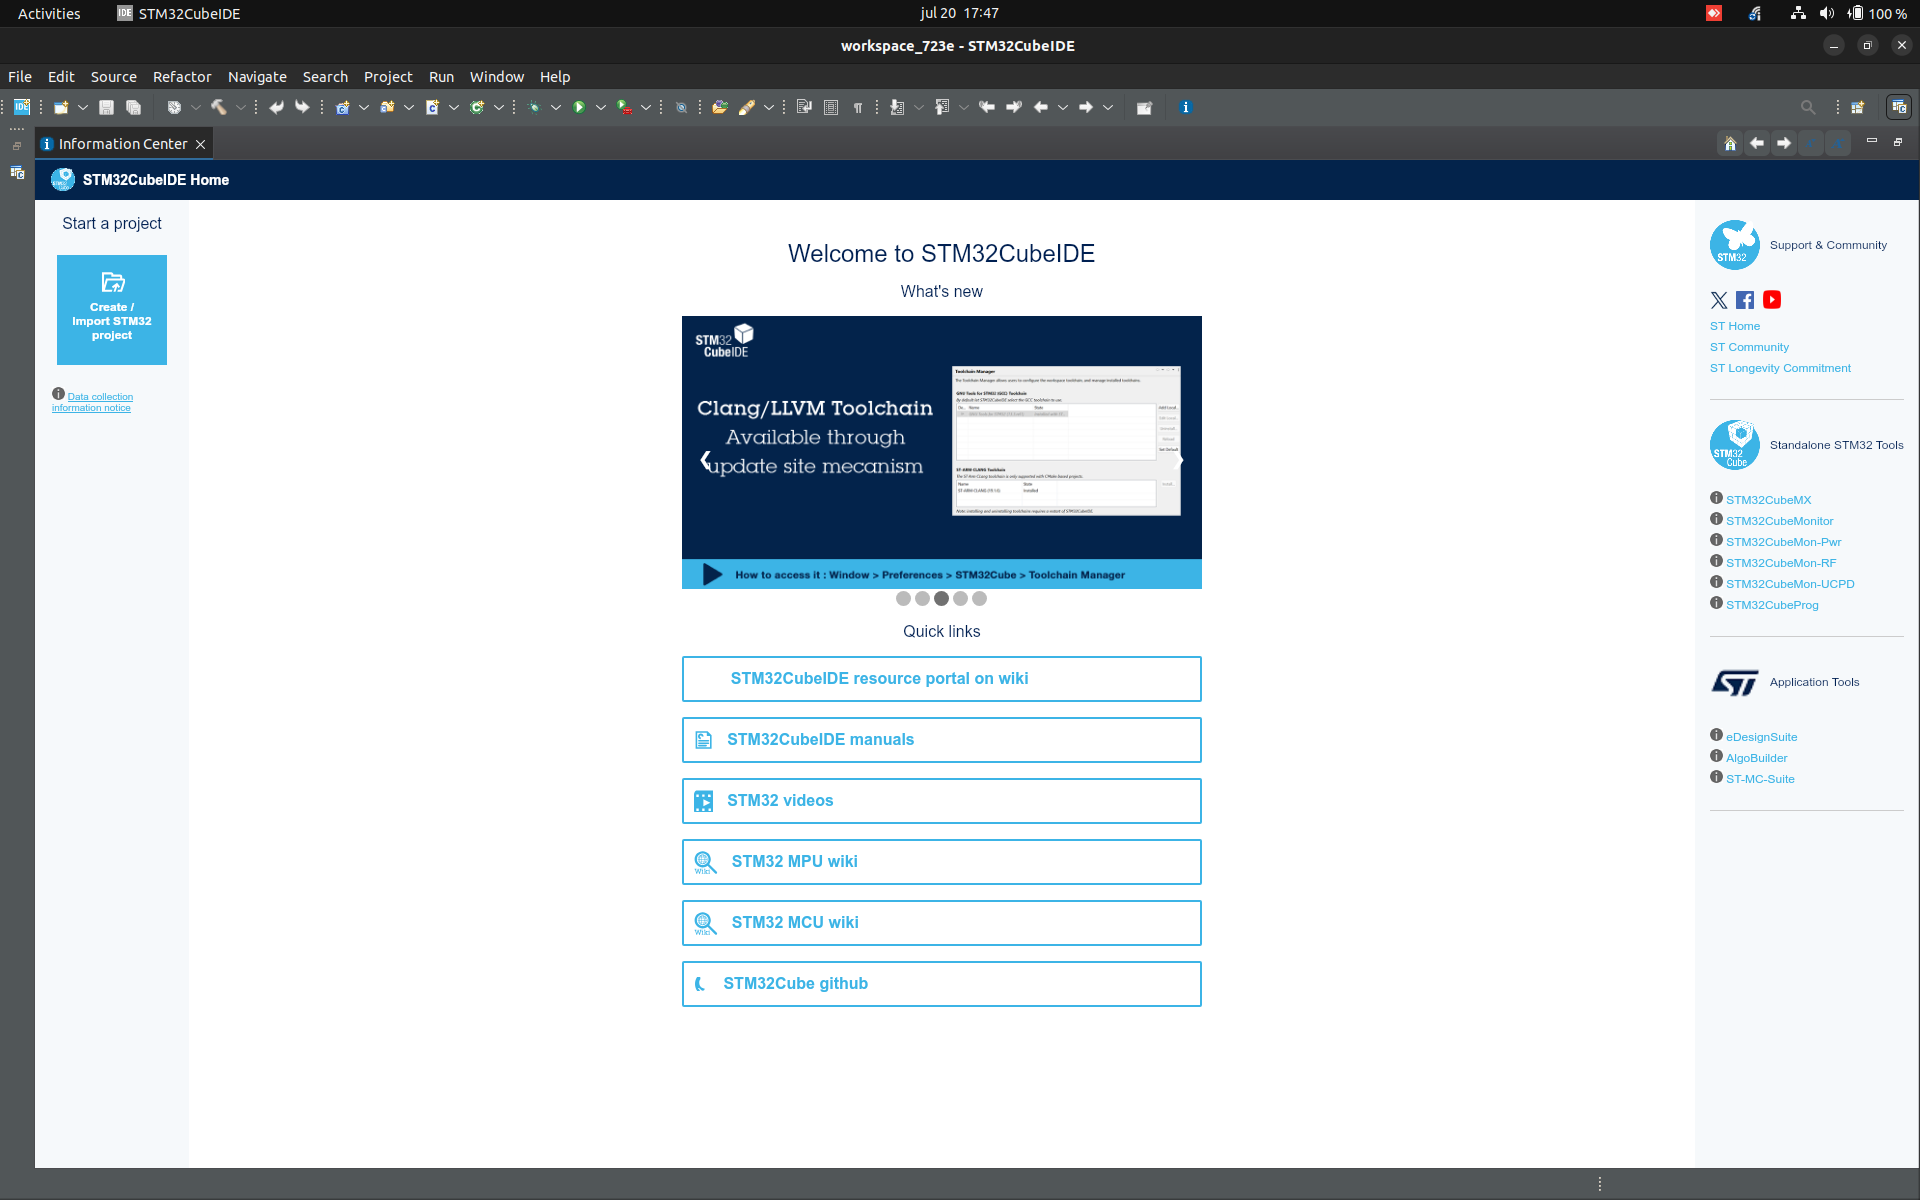
\includegraphics[width=\textwidth]{res/scrn_01_startup.png}
                        \caption{Ventana inicial de la aplicación}
                        \label{fig:scrn_01_startup}
                    \end{figure}
                \item Creamos un nuevo proyecto con \texttt{File > STM32 Project Create / Import}.
                \item Seleccionamos \texttt{STM32CubeIDE Empty Project} (\Cref{fig:scrn_02_project})
                    
                    \begin{figure}
                        \centering
                        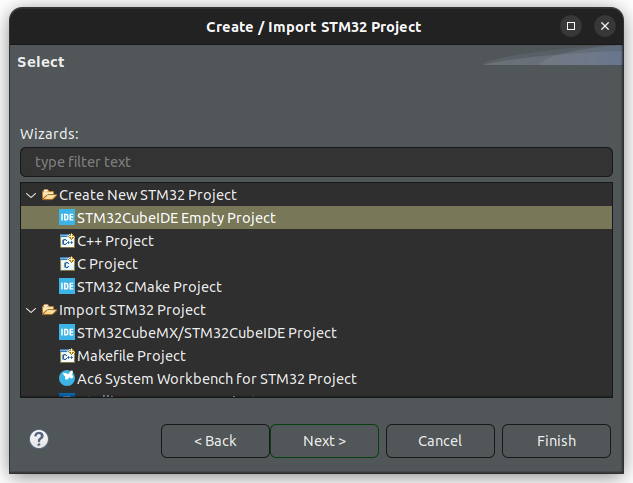
\includegraphics[width=\textwidth]{res/scrn_02_project.png}
                        \caption{Creación de proyecto}
                        \label{fig:scrn_02_project}
                    \end{figure}

                \item En \texttt{Board Selector}, buscar \texttt{723e} y seleccionar la única placa disponible (\Cref{fig:scrn_03_boardsel}).
                                    
                    \begin{figure}
                        \centering
                        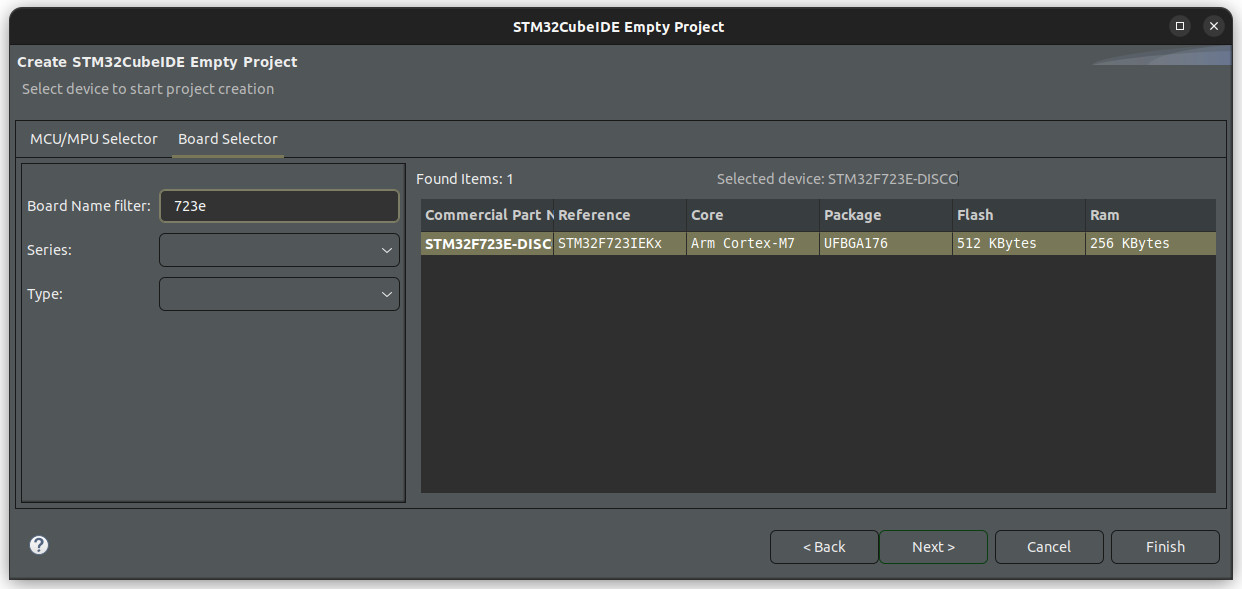
\includegraphics[width=\textwidth]{res/scrn_03_boardsel.png}
                        \caption{Selección de placa}
                        \label{fig:scrn_03_boardsel}
                    \end{figure}

                \item Finalmente, dar un nombre al proyecto y terminar (\Cref{fig:scrn_04_namesel}).
                    
                    \begin{figure}
                        \centering
                        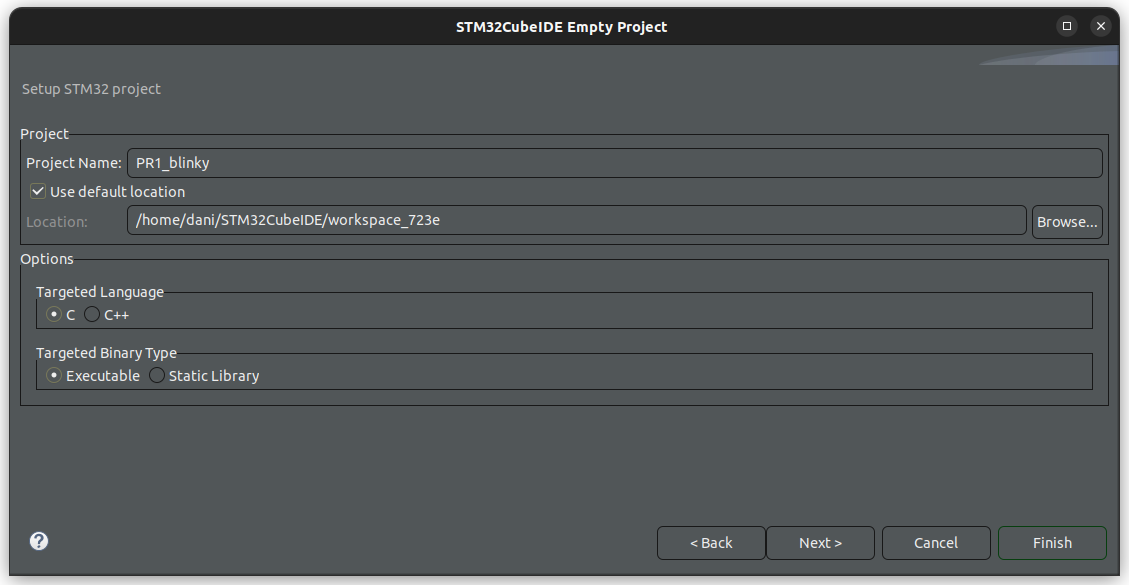
\includegraphics[width=\textwidth]{res/scrn_04_namesel.png}
                        \caption{Selección de nombre de proyecto}
                        \label{fig:scrn_04_namesel}
                    \end{figure}
            \end{enumerate}

        \subsubsection{Depuración del proyecto}
        
            Ahora deberíamos tener un proyecto en blanco para trabajar (\Cref{fig:scrn_06_structure}). Antes de nada, vamos a probar que la conexión con la placa funciona, y podemos compilar y depurar el proyecto. Para ello:

                \begin{figure}
                    \centering
                    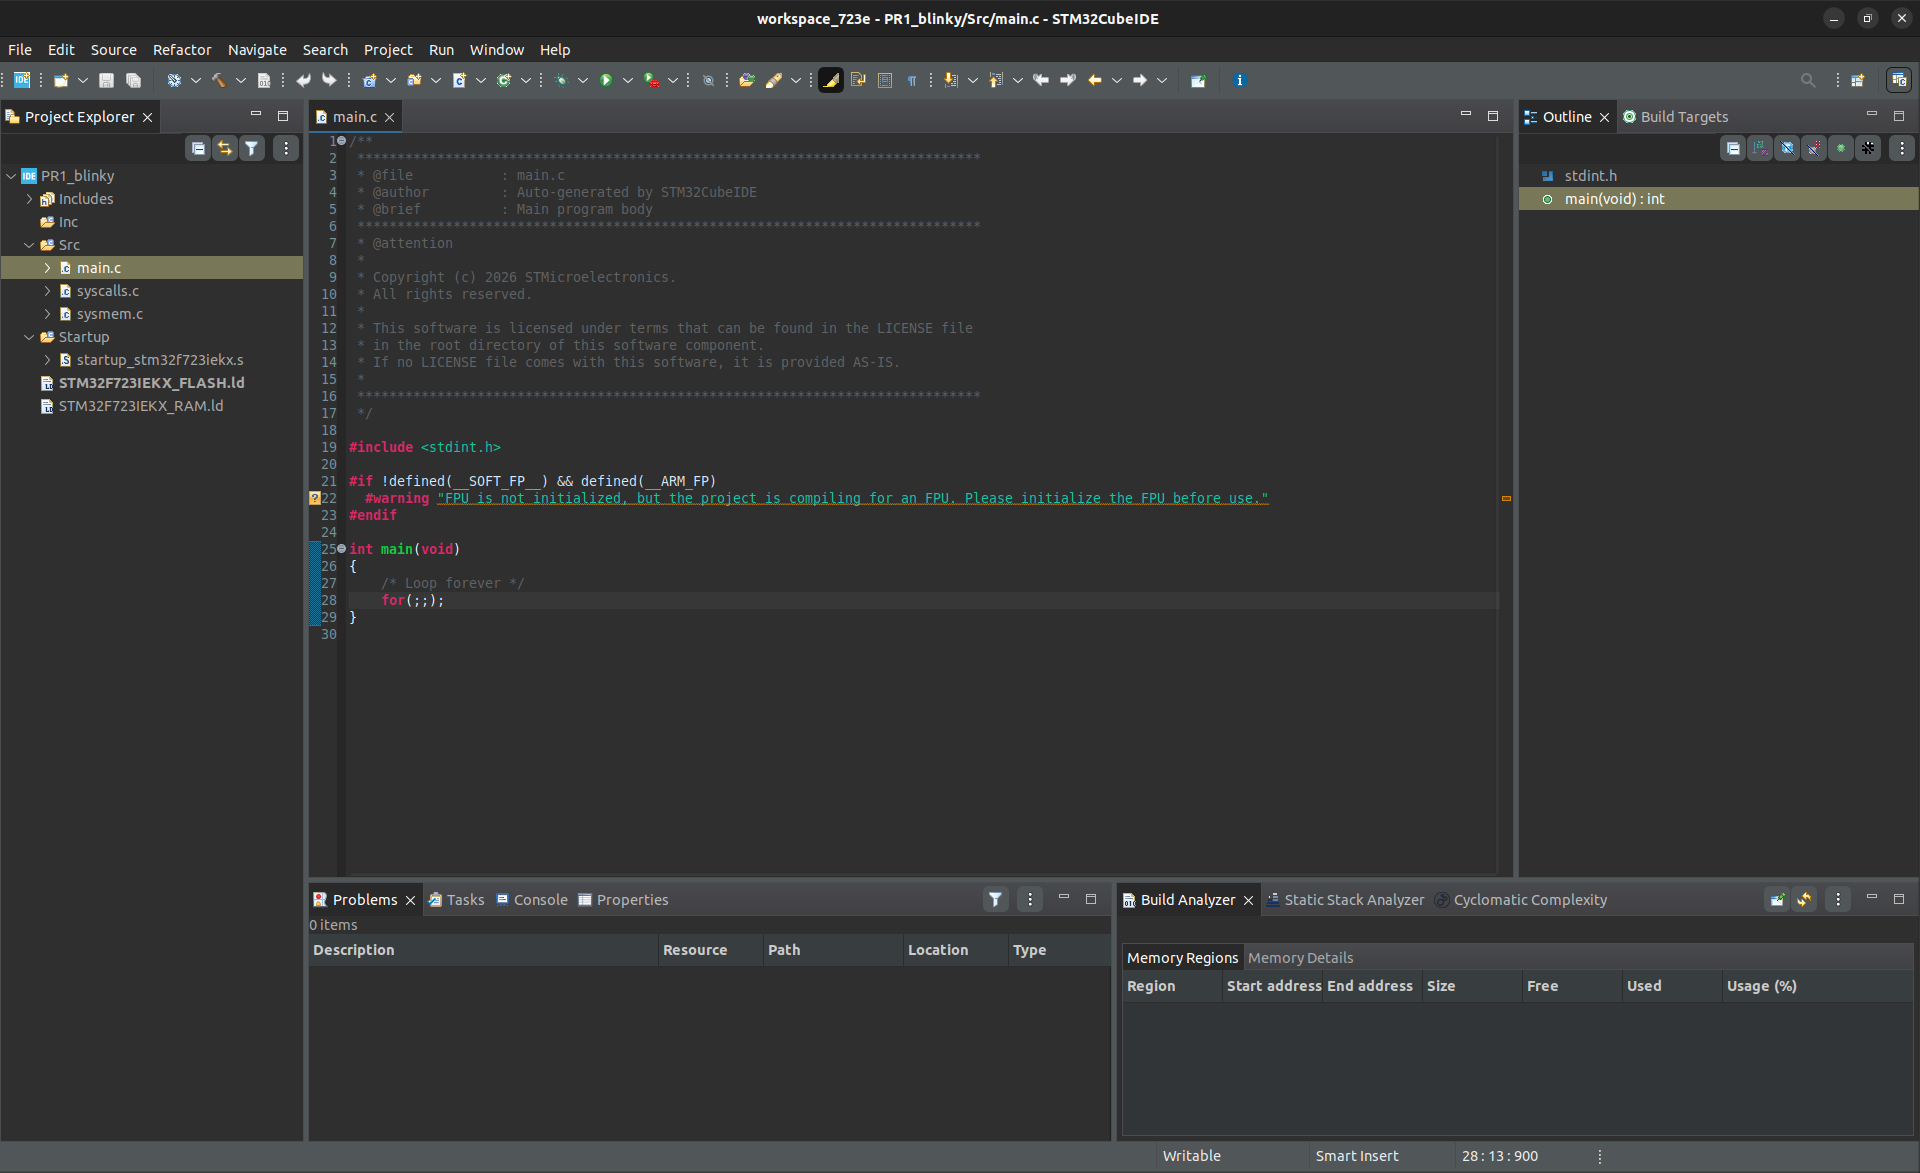
\includegraphics[width=\textwidth]{res/scrn_06_structure.png}
                    \caption{Aplicación por defecto}
                    \label{fig:scrn_06_structure}
                \end{figure}

            \begin{enumerate}
                \item Haz doble click en la carpeta \texttt{Src} dentro de tu proyecto, y luego, en \texttt{main.c}. 
                \item Con el archivo abierto, haz click en el martillo (build) que se encuentra en la barra superior de tareas. Verás el log de compilación en la terminal (\Cref{fig:scrn_07_build}).
                
                    \begin{figure}
                        \centering
                        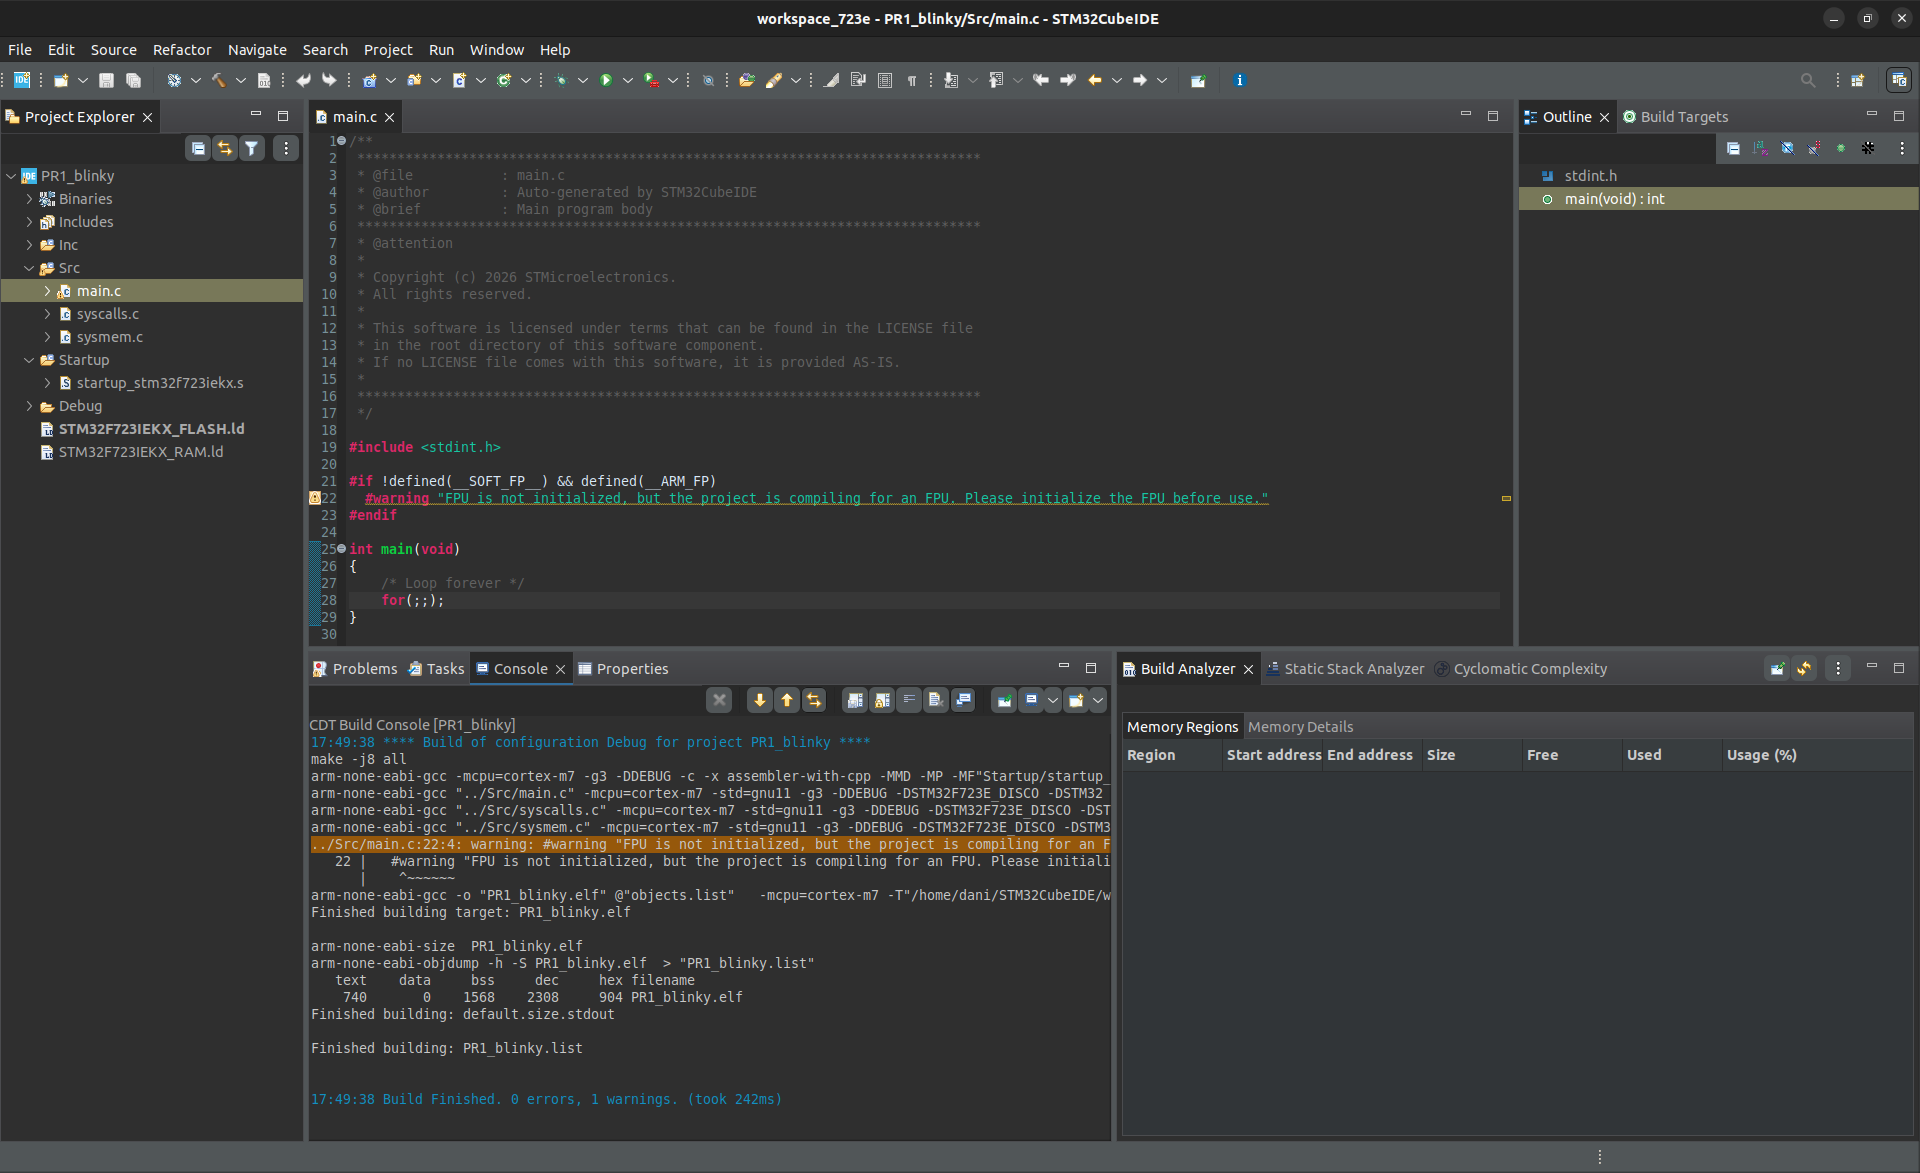
\includegraphics[width=\textwidth]{res/scrn_07_build.png}
                        \caption{Log tras construir la aplicación}
                        \label{fig:scrn_07_build}
                    \end{figure}

                \item Finalmente, y si no ha habido problemas, haz click en el icono de depuración (debug) en la misma barra superior (el bichito verde).
                \item Acepta la configuración de depuración por defecto (\Cref{fig:scrn_08_debugsel}) y vuelve a aceptar cuando pida cambiar a la vista de depuración.
                
                    \begin{figure}
                        \centering
                        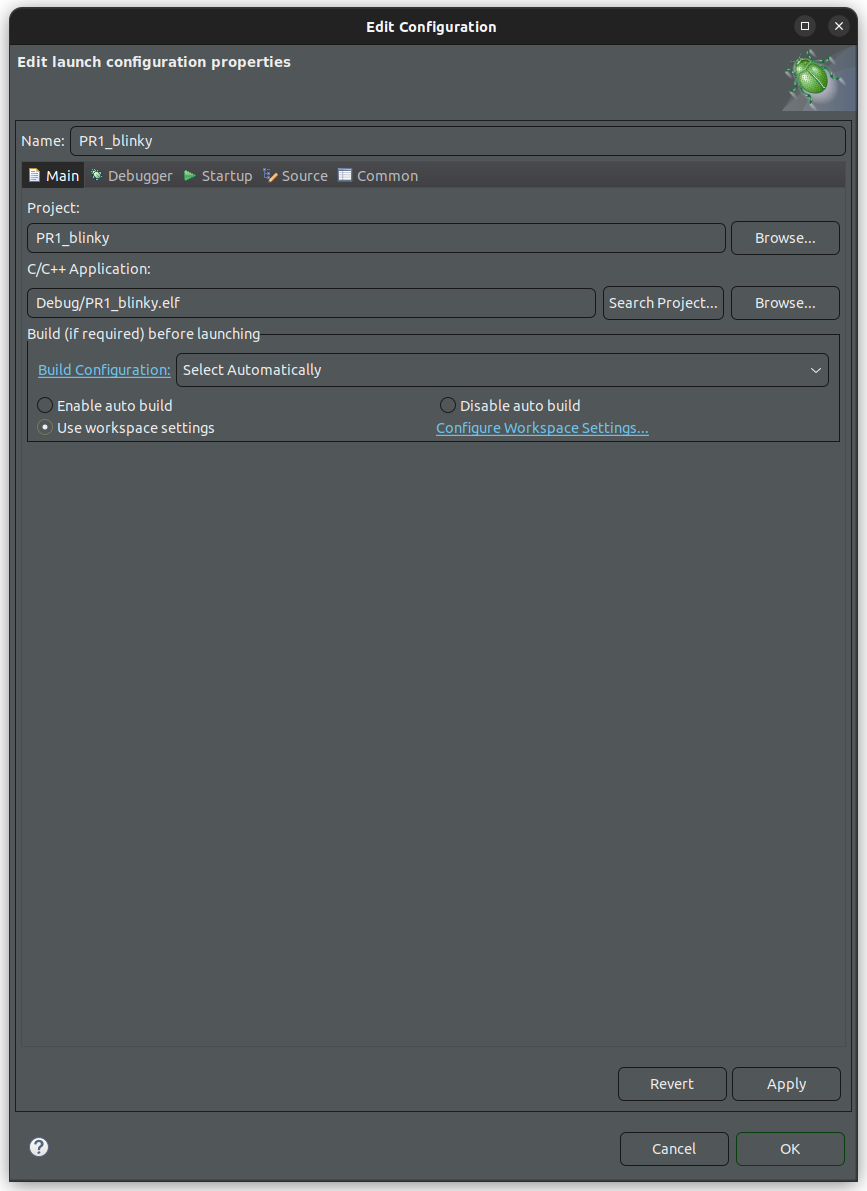
\includegraphics[width=\textwidth]{res/scrn_08_debugsel.png}
                        \caption{Selección de depuración por defecto}
                        \label{fig:scrn_08_debugsel}
                    \end{figure}
            \end{enumerate}

            Ahora puedes depurar el proyecto poco a poco. Entre otras, el depurador permite:
                \begin{itemize}
                    \item Ir paso a paso por las líneas de código.
                    \item Colocar \emph{breakpoints} para parar la ejecución al llegar a ciertas líneas.
                    \item Inspeccionar el contenido de los registros del procesador.
                    \item Inspeccionar el contenido de los registros de los diferentes periféricos.
                    \item Inspeccionar el contenido de la memoria.
                \end{itemize} 

            Se recomienda explorar todas estas funcionalidades, que se pueden ver en la \Cref{fig:scrn_11_debugpersonalized}.

                \begin{figure}
                    \centering
                    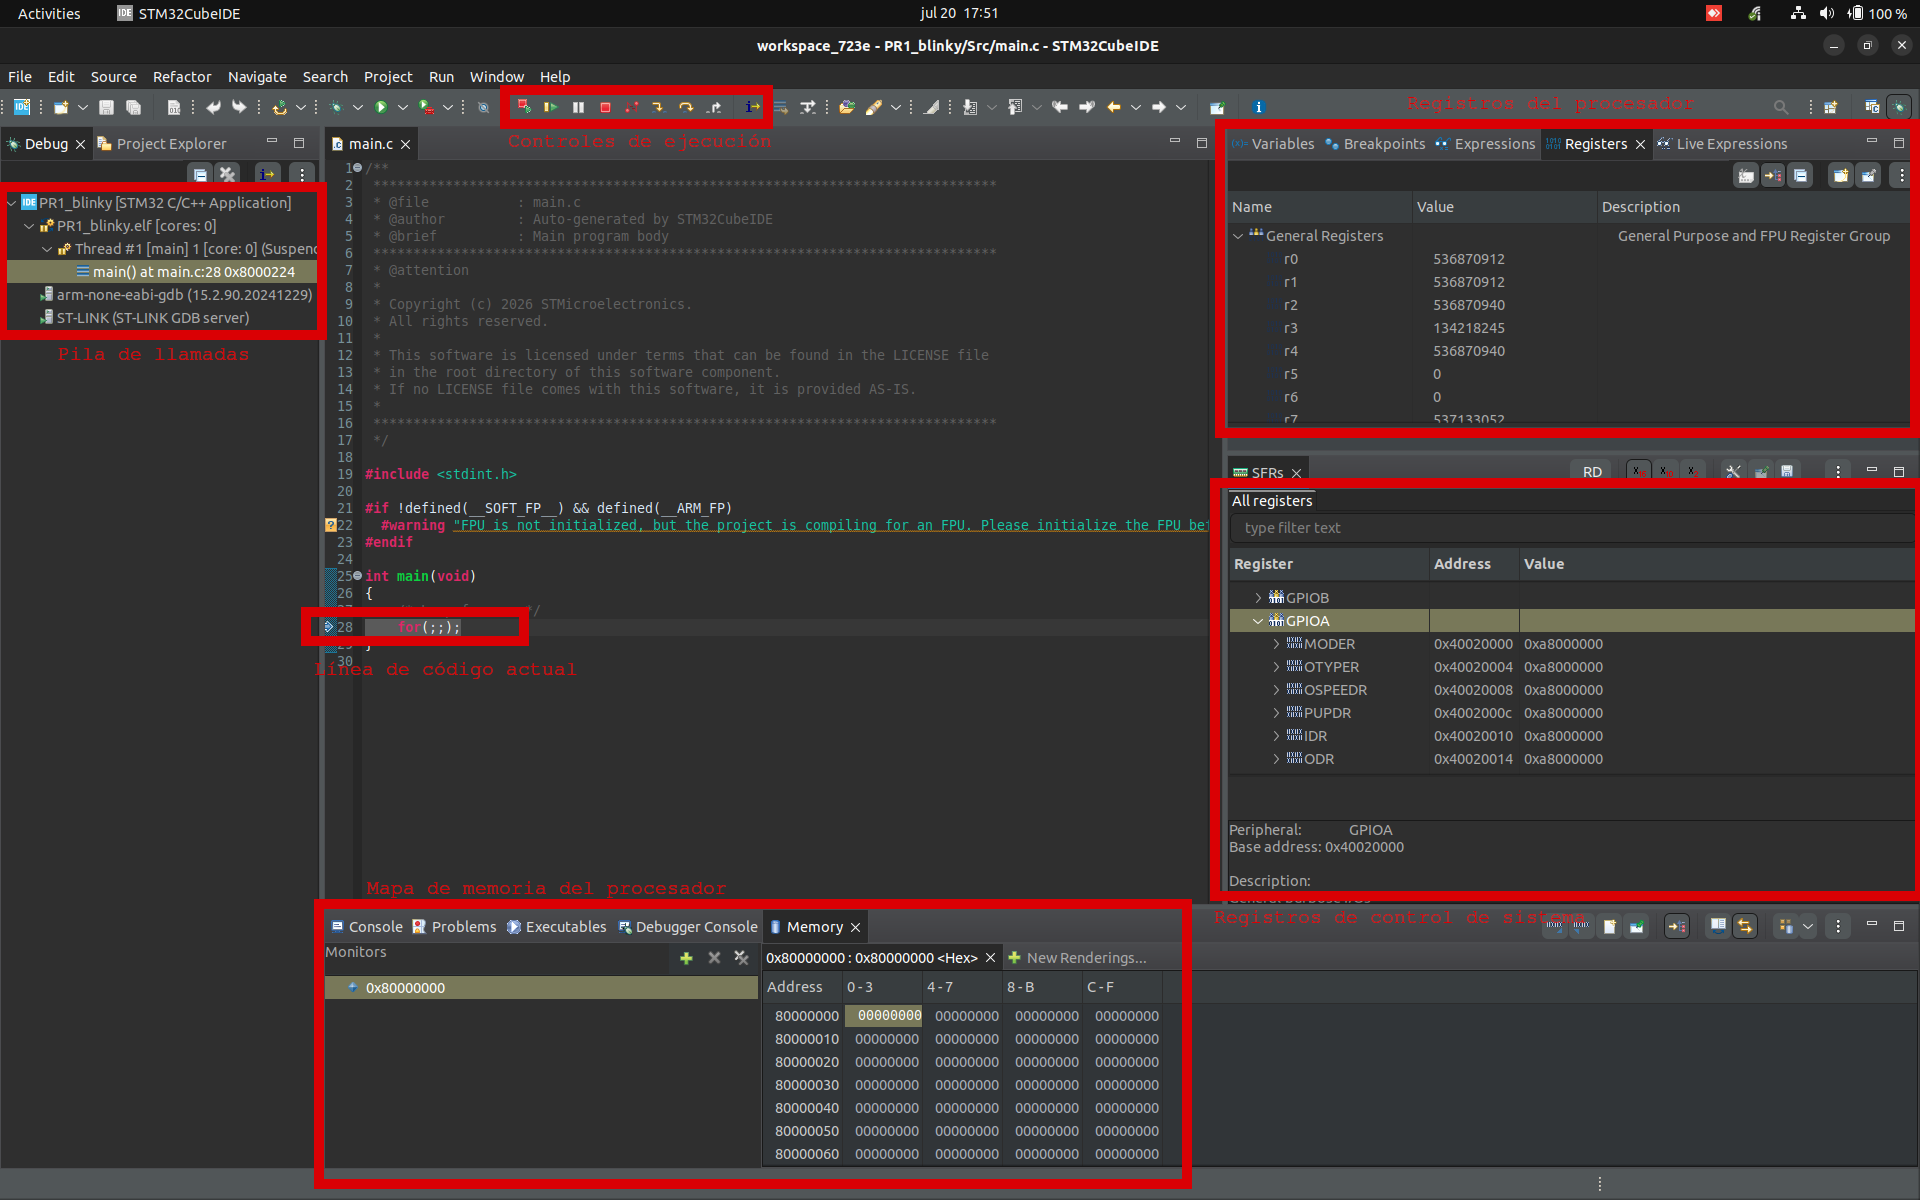
\includegraphics[width=\textwidth]{res/scrn_11_debugpersonalized.png}
                    \caption{Ventana de depuración personalizada}
                    \label{fig:scrn_11_debugpersonalized}
                \end{figure}
            
        \subsubsection{Desarrollo del proyecto}

            Finalmente, debemos programar nuestro código para encender el LED. Para ello, habrá que escribir en las direcciones concretas de los registros de GPIO, en este caso de GPIOA-PIN7. Recuerda que la documentación de los registros disponibles está en \REFMAN[6.4].

            \begin{itemize}
                \item Configurar GPIOA-PIN7 como salida en \REG{MODER}.
                \item Poner el pin en tipo \emph{push-pull} en \REG{OTYPER}.
                \item Configurar la velocidad a alta en \REG{OSPEEDR}.
                \item Deshabilitar las resistencias en \REG{PUPDR}.
                \item Finalmente, se podrá escribir el valor del led (0/1) a través de \REG{ODR}. Otra opción es escribir directamente al registro \REG{BSRR}, que tiene la ventaja de evitar lecturas o escrituras múltiples (aunque para nuestro caso no afecta en nada).
            \end{itemize}

            Adicionalmente, tenemos que activar el reloj del periférico GPIOA a través del registro \REG{RCC\_AHB1ENR} (\REFMAN[5.3.10]). La dirección base la podemos consultar en \REFMAN[1.6.2].

            Quizá te quede la pregunta de cómo narices escribo yo en una dirección de memoria concreta... la respuesta son... ¡punteros!

            \begin{lstlisting}
                //Imaginemos que quiero escribir en la dirección 0x40020000
                //justo en los bits 14-15
                // (por lo que sea)
                
                //borro configuración actual (máscara con ceros en las posiciones de interés)
                * ((uint32_t *) (0x40020000)) &= ~(0b11 << (7*2));
                //pongo la configuración que me interesa
                * ((uint32_t *) (0x40020000)) |=   0b01 << (7*2);
            \end{lstlisting}
            
            Aprovecha también esta función para hacer que parpadee cada cierto tiempo:

            \begin{lstlisting}
                void delay(int loops) {
                    for (int i = 0; i < loops; i++) {
                        __asm("nop");
                    }
                }
            \end{lstlisting}

            Nuestra función \lstinline|main.c| tendrá por tanto esta pinta:

            \begin{lstlisting}
                int main(void)
                {
                    //activar reloj de GPIOA en RCC_AHB1ENR
                    //configurar Pin0-GPIOA como salida
                    //configurar Pin0-GPIOA modo push-pull
                    //configurar Pin0-GPIOA velocidad alta
                    //configurar Pin0-GPIOA con pullup/down desactivado

                    /* Loop forever */
                    for(;;) {
                        //encender LED
                        delay(1000000);
                        //apagar LED
                        delay(1000000);
                    }
                }
            \end{lstlisting}

    \subsection{Para hacer más}

        Busca el GPIO del botón de la placa, configúralo en modo entrada, y haz que el LED se encienda o apague cada vez que se pulse el botón, en lugar de hacerlo de manera automática.


\end{document}